\section{Data set}

The ASK corpus (\emph{andrespråkskorpus}) was presented in 2006
\autocite{tenfjord06}. The corpus contains Norwegian learner essays from two
different language tests: \emph{Språkprøven i norsk for voksne innvandrere}
and \emph{Test i norsk – høyere nivå}, which test proficiency at the B1 and
B2 levels, respectively. Following the naming in
\textcite{carlsen2012proficiency}, we will refer to these tests as the
\emph{IL test} (Intermediate Level, ``Språkprøven'') and the \emph{AL test}
(Advanced Level, ``Høyere nivå'').

The corpus contains 1736 texts\footnote{In
\textcite{carlsen2012proficiency,malmasi15,malmasi17}, it's reported that it
contains 1700 texts.}. Each document includes metadata such as the writer's
L1: one of German, Dutch, English, Spanish, Russian, Polish,
Bosnian-Croatian-Serbian, Albanian, Vietnamese and Somali. All texts from
seven of these language backgrounds, 1212\footnote{Reported to be 1222 in
\textcite{carlsen2012proficiency}.} in total, have been assigned a CEFR
score. In particular, all texts except those written by people with Dutch,
Bosnian-Croatian-Serbian or Albanian as L1 have a CEFR score. The CEFR labels
are available since work by \textcite{carlsen2012proficiency}, and were not
included at the corpus' initial release.

The corpus also includes 200 texts written by native Norwegian speakers as a
control corpus. The total number of word and punctuation tokens in the full
corpus, including the control corpus, is approximately 770,000. Restricting
the corpus to the 1212 documents with CEFR score, the number of tokens is
approximately 487,000 in total. Other metadata included, apart from L1 and
CEFR score, are the test level the essays were written for, what topic the
essay is about, the learner's country of origin, age, gender and more.


\section{Data split}

At the start of the project, the dataset was split into a training set and a
test set in a 90:10 proportion. Ideally, the train and test sets would have
the same distribution of classes, but the limited amount of data made this
more difficult. As can be seen from figure \ref{lang-vs-cefr}, 15 of the
combinations language vs. proficiency label consist of only three or fewer
documents.

\begin{figure}
  \centering
  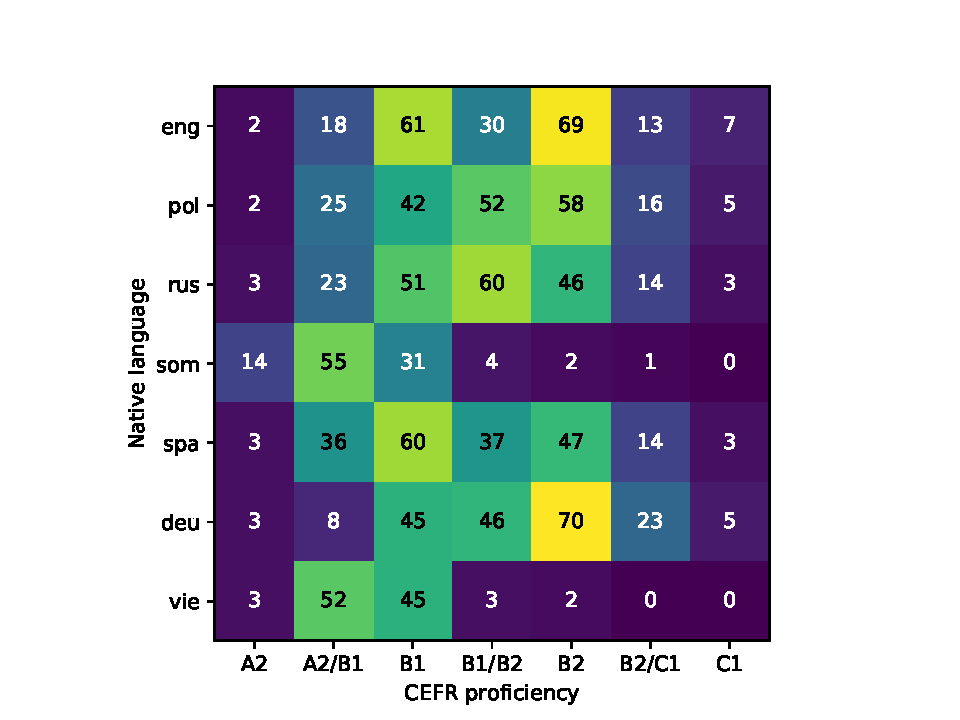
\includegraphics[height=0.3\textheight]{lang_vs_cefr}
  \caption{The distribution of proficiency scores for each L1}
  \label{lang-vs-cefr}
\end{figure}
 
\begin{figure}
  \centering
  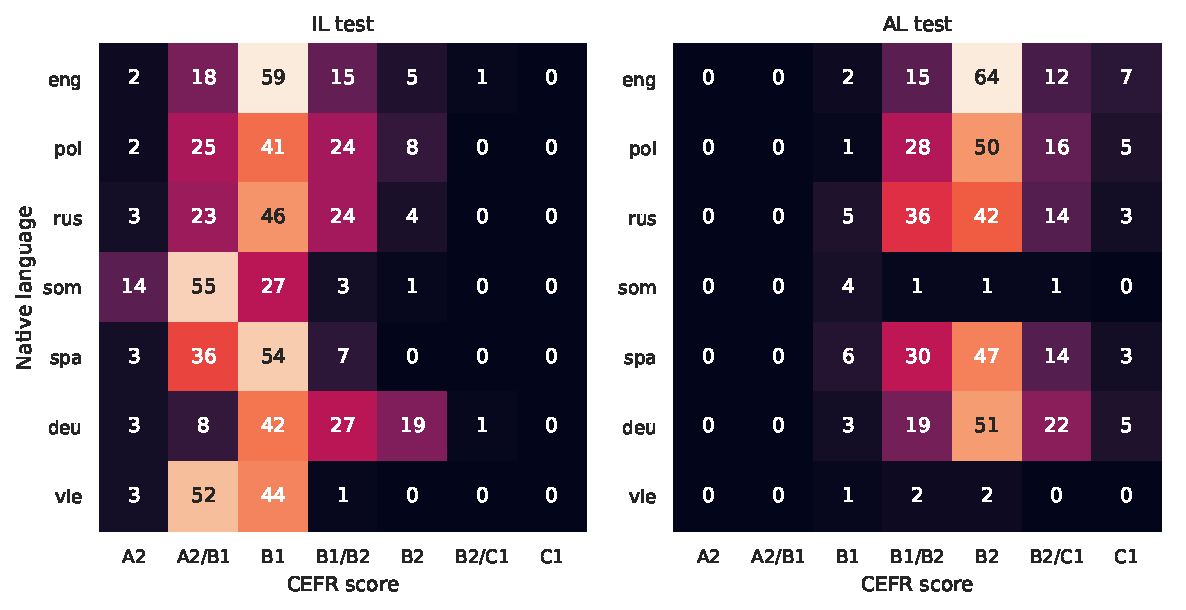
\includegraphics[width=\textwidth]{testlevel_lang_vs_cefr}
  \caption{L1 versus CEFR score for each test level}
  \label{testlevel-lang-vs-cefr}
\end{figure}
 
\subsection{Metadata}

Analysis of the data set was carried out in order to find correlations
between different metadata. Knowing that the documents stem from two
different language tests that measure different levels of proficiency, the
data set was split into two along the \emph{Test level} label, and then broken
down by language and proficiency again. Figure \ref{testlevel-lang-vs-cefr}
shows that the test levels have different distributions of proficiency. Note
also that two language groups are underrepresented at the B2 test level
(\emph{AL test}), namely Somali and Vietnamese, which have seven and five
essays in the B2 test level, respectively. All other combinations of L1 and
test level contain exactly 100 essays. This partly explains the low average
proficiency of Somali and Vietnamese speakers apparent in figure
\ref{lang-vs-cefr}. The difference compared to the other language groups is
not as salient when looking only at the B1 test level (\emph{IL test}) data.

Another interesting variable is the essay topic. There is generally a strong
correlation between topic and vocabulary, and not accounting for this may
lead to a model picking up the wrong signal. Since the data is collected from
two different language tests, we might expect the distribution of topics to
differ between the test levels, and this is the case. Looking at the ten most
common topics in the data (table \ref{texts-per-topic}), several are only
present on one test level.

There is also a difference in granularity. There are 52 topics in ``Høyere
nivå'' and only 38 topics in \emph{IL test}, even though there are more
documents in the latter test level (512 vs. 700). This also means that the
topics within each test level have different support. The median number of
documents for a topic in \emph{AL test} is 5 (mean 9.8), while it is 11 in
\emph{IL test} (mean 18.4). This also explains the overrepresentation of
\emph{IL test} in the table of top ten topics.

It is seen that some topics in the diagram consist of several sub-topics.
However, the number of individual sub-topics is 62, still quite large.
However, they seem to be more evenly distributed across essays. The median
number of documents for a sub-topic, for both test levels, is 25 (mean 34.8).
13 sub-topics are represented in 5 or fewer documents.

\begin{table}
  \centering
  \begin{tabular}{lrrr}
    \toprule
    Topic                    & AL test & IL test & Total \\
    \midrule
    telefon                  &      37 &      64 &   101 \\
    bolig                    &       0 &      83 &    83 \\
    familie helse vekt       &      59 &       0 &    59 \\
    tid                      &       2 &      51 &    53 \\
    natur norge              &       0 &      48 &    48 \\
    folk relasjoner vennskap &       0 &      45 &    45 \\
    tradisjoner flytting     &       0 &      38 &    38 \\
    barn                     &       3 &      32 &    35 \\
    kultur norge             &       0 &      34 &    34 \\
    media                    &       0 &      31 &    31 \\
    \bottomrule
  \end{tabular}
  \caption{Number of texts in each test level for top 10 topics}
  \label{texts-per-topic}
\end{table}

Document lengths have been seen to correlate with essay score in other
studies such as \textcite{vajjala17}. To see the relationship between these
variables in ASK, we again break down the data into the two test levels. One
group, \emph{B2/C1} CEFR score within \emph{IL test}, was excluded due to
having fewer than ten documents. Looking at figure
\ref{testlevel-lengths-per-cefr}, two relations are apparent. Essays in the
\emph{AL test} test level are generally longer than in \emph{IL test}, and
within each test level the higher scoring essays are generally longer. Note
that even for the same CEFR score, the essays from the higher test level are
considerably longer. As an example, consider the \emph{B1/B2} score, which is
the most evenly distributed between the two test levels (101 essays in
\emph{IL test}, 131 in \emph{AL test}). More than 75~\% of these texts on
the lower test level have fewer than 400 tokens, and more than 75~\% on the
higher level are longer than 400 tokens.


\begin{figure}
  \centering
  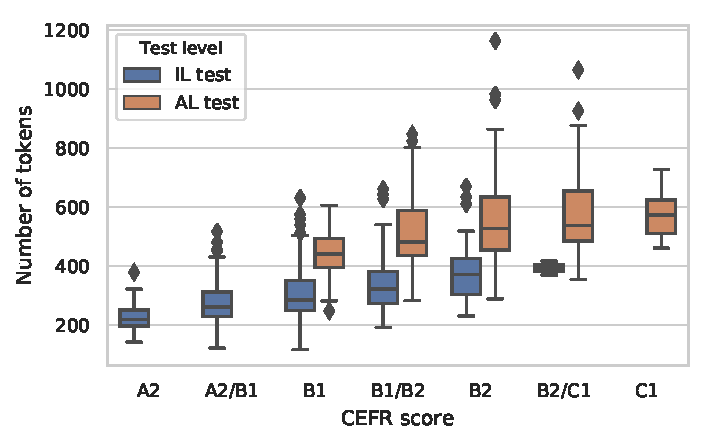
\includegraphics[width=\textwidth]{testlevel_lengths_per_cefr}
  \caption{Distributions of essay lengths for CEFR scores on each test level}
  \label{testlevel-lengths-per-cefr}
\end{figure}
 